\section{\Moire{}}
\label{sec:system}

\Moire{} is a browser tool. It is also the reason the previous three sections
exist: every bound in them was forced by something an author could do with a
slider and we could not draw fast enough or correctly enough. This section
describes the program, and concentrates on the five decisions that the field
formulation makes available and that we would not have found otherwise.

\subsection{One pass, twelve slots, compiled once}

The whole picture is a single full-screen fragment program. There is no geometry
beyond one quad, no texture, no render target, and no rasterization of any layer
into any buffer. The program is written in Three.js's shading
language~\cite{ThreeJS} and runs through WebGPU~\cite{WebGPU}; TSL matters here
only because it lets the same expression tree be assembled in TypeScript, which is
how the CPU twin of \S\ref{sec:inverse} stays a twin.

A layer is $19$ uniforms. Nine describe the family---type, previous type, morph
parameter, spacing, phase, side count, per-member offset, per-member rotation,
line count---and the rest describe its appearance and placement. Crucially there
are always \emph{twelve} of these slots, allocated and compiled at startup, each
gated by an \texttt{active} uniform. Adding a layer writes uniforms. Deleting or
hiding one writes $\texttt{active}=0$. Neither touches the node graph.

This is a small decision with a large consequence, and we got it wrong first. The
natural way to write the renderer is to build the shader from the current layer
list, which means every add, delete and hide rebuilds it. In WebGPU a rebuild is a
pipeline creation, and pipeline creation is tens to hundreds of milliseconds during
which the canvas cannot present. The result is a tool that stutters exactly when
an author is composing---the moment when they are most likely to be exploring
rather than committing. Fixing the layer count and paying for twelve unconditionally
costs a few branches per pixel and makes layer count free. Frames are then driven
by a dirty flag on the store, coalesced to one render per animation frame.

\paragraph{The one exception, and how it is paid for.}
Exactly one edit changes the program: a layer's field \emph{expression}, which is
compiled into the shader rather than interpreted by it (\S\ref{sec:exprs}).
Three things hide the rebuild: it is per slot, so eleven layers are undisturbed;
it is debounced by $220$\,ms, longer than the gap between keystrokes; and the
renderer holds the last presented frame across the build while the field editor's
live preview runs on the CPU evaluator, so the author never waits on the GPU to
see what they typed.

\subsection{The stroke floor}
\label{sec:zoom}

A family is a set of curves of zero width; ink comes from thresholding the
distance field. Given a stroke thickness $t$, write $\mathrm{pixel}=1/\mathrm{zoom}$
for the world size of a pixel and set
\begin{equation}
  h=\max\!\left(\tfrac{t}{2},\; 1.15\,\mathrm{pixel}\right),
  \qquad
  \varepsilon = 0.7\,\mathrm{pixel},
  \label{eq:stroke}
\end{equation}
then $\alpha(d)=1-\mathrm{smoothstep}(h-\varepsilon,\,h+\varepsilon,\,d)$.

The floor $1.15\,\mathrm{pixel}$ is what keeps a zoomed-out pattern from
disintegrating. Without it, a hairline family at low zoom has strokes narrower
than the sample spacing, and the picture breaks into speckle that is visually
indistinguishable from the inversion failure of \S\ref{sec:inverse}---the
two are easily attributed to each other. With it, the stroke can never be
thinner than about a pixel, and the fringes survive (Figure~\ref{fig:zoom}).

To quantify what the floor does, take a spiral over a displaced circle family,
fix a world window, and render it over $\zoomDecades$ decades of zoom twice:
once at one sample per pixel, as the shader does, and once at $\zoomRefSamples$
samples per pixel as a prefiltered reference. Each rule is compared against the
properly sampled version of \emph{its own} intent, so that sampling error is
isolated from any difference in what was being drawn. At the coarsest zoom,
where one carrier period is $\zoomCoarsestPeriod$\,px, the standard deviation
of the per-pixel ink error is
\begin{center}\small
\begin{tabular}{@{}lrr@{}}
  \toprule
  & worst noise & at coarsest zoom \\
  \midrule
  with the floor            & $\zoomFloorNoise$   & $\zoomFloorNoiseCoarse$ \\
  floor removed             & $\zoomNoFloorNoise$ & $\zoomNoFloorNoiseCoarse$ \\
  phase residual, no floor  & $\zoomValueNoise$   &---\\
  \bottomrule
\end{tabular}
\end{center}---a factor of $\zoomNoiseRatio$. So the floor does suppress the speckle, and by a
lot. But the same experiment prices it: even sampled perfectly, the clamped stroke
lays down up to $\zoomFloorInkGain$ more ink per pixel than the hairline it stands
in for, because a stroke held at a pixel wide inside a period that is narrower than
that must overlap itself.

The floor, in other words, is not an antialiasing method. It converts an unbiased
and very noisy estimate of the pattern into a biased and nearly noiseless one, and
it is the right trade only because a moir\'e is read as structure rather than as
tone: a frame that is uniformly too dark preserves the pattern, and a peppered
one destroys it. The unbiased low-noise answer is the analytic mean of the
family over the pixel, which for a walking family we do not have---the open
problem of \S\ref{sec:future}. The floor predates this characterization; the
measurement is what identified which of the two errors it chooses.

Two things about \eqref{eq:stroke} are only correct because of the field view.
First, $h$ is a \emph{world} distance, so it must be compared against a world
distance, which is why the gradient divide of Table~\ref{tab:catalog} is not
optional: applied to a phase residual, the floor guarantees nothing, because a
phase unit is not a length. Second, having a hard $h$ means we know in advance
which distances cannot matter. Anything beyond $h+\varepsilon$ is fully
transparent. The solver of \S\ref{sec:inverse} is therefore not asked for
$\min_n d_n$; it is asked whether any $d_n$ falls below $h+\varepsilon$, and is
free to \emph{prove} the rest away without evaluating them. The guard and the skip
rule are the same idea seen from two ends.

\begin{figure*}[t]
  \centering
  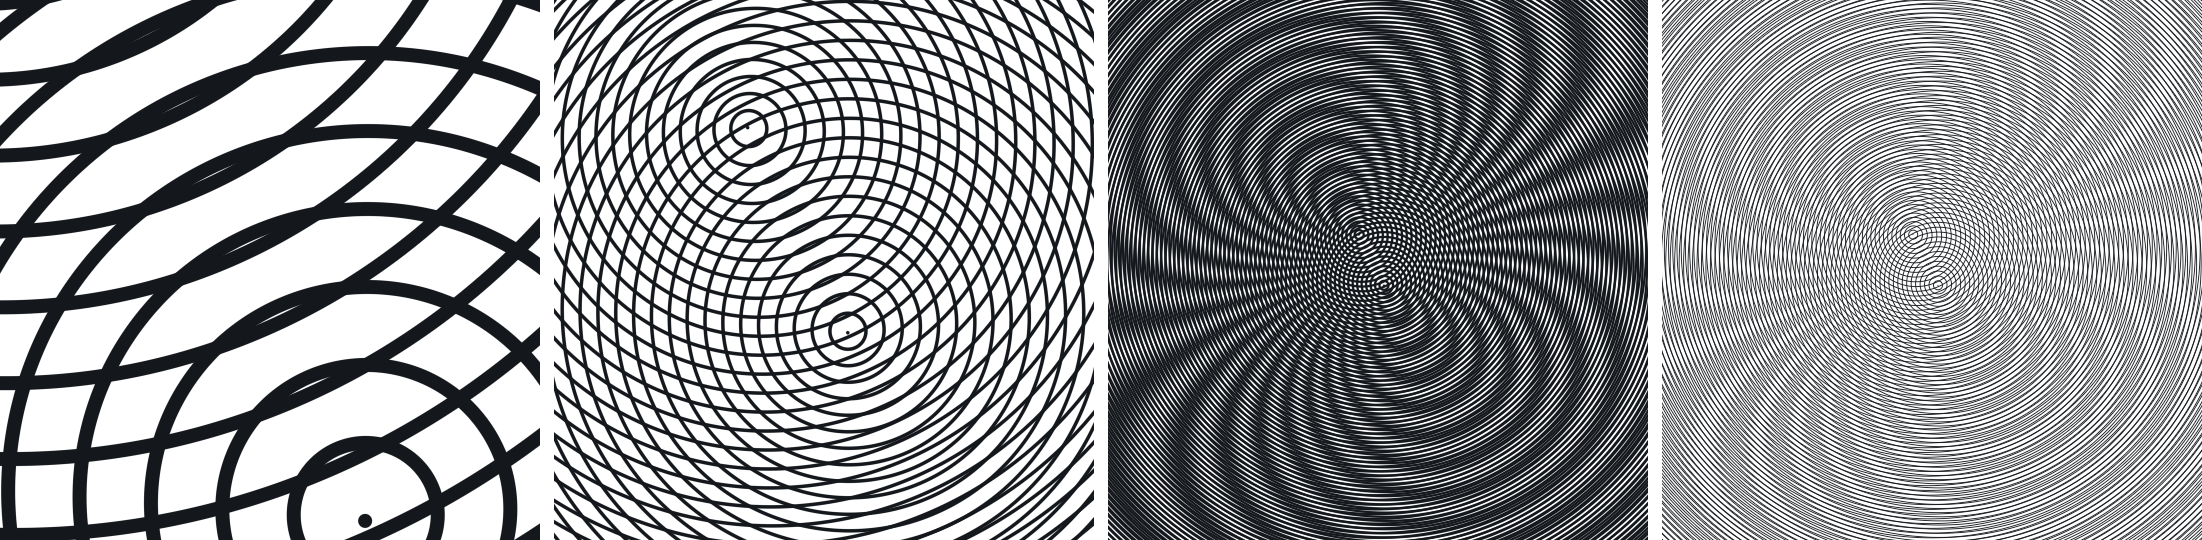
\includegraphics[width=\linewidth]{figures/zoom.png}
  \panelrow{0.24523}{0.00636}{%
    (a) zoom $2$,
    (b) zoom $1$,
    (c) zoom $0.25$,
    {(d) zoom $0.25$, no floor}}
  \Description{Four square panels of the same black-on-white scene at falling zoom.
  The first shows a bold open weave of ring arcs from two centers on the frame's
  diagonal; the second shows the whole two-center rosette, its rings crossing in a
  lens pattern; the third packs the same rosette into a dense dark pinwheel of spiral
  fringe arms; the fourth is the third panel again but washed out to pale gray and
  visibly speckled, with the fringe arms no longer readable.}
  \caption{\figlead{One scene over an eightfold zoom range, with and without
  the stroke floor.}
  Two walking circle families---the tool's default preset, recomposed with its
  centers on the frame's diagonal.
  \textbf{(a--c)}~zoom $2$,
  $1$ and $0.25$. Nothing is resampled between them: each is the same pair of scalar
  fields evaluated on its own grid, so there is no mip level to choose, no filter
  kernel to widen, and no resolution at which the pattern was ever committed. Stroke
  thickness is a \emph{world} quantity and is the same number in all four panels,
  which is why the strokes get thinner on screen as the zoom falls. \textbf{(d)}~the
  same frame as (c) with the stroke floor of \eqref{eq:stroke} removed. All four are
  rendered at one sample per pixel, exactly as the shader does, so (c) and (d) differ
  in one constant and nothing else. The floor is what keeps the fringe system in (c);
  without it the sub-pixel strokes are hit or missed and the pattern goes pale and
  grainy. The floor's cost, the ink it adds, is measured in
  \S\ref{sec:zoom}. (The table there uses a plainer pair, a spiral over rings, since
  the third rule under test needs a family with a closed-form phase.)}
  \label{fig:zoom}
\end{figure*}

\subsection{Continuous transitions between families}

Switching a layer from circles to hexagons is a change of $\ph$, and the direct
implementation of that is a jump. Authors read a jump as breakage, and more
importantly they cannot see \emph{what} changed, which is precisely the thing a
tool for studying interference should show.

So the slot carries two family codes and a mix parameter: the shader evaluates the
distance under both the old family and the new one and interpolates the
\emph{distances}, easing the mix over $280$\,ms with a cubic. Interpolating
distances rather than images means there is one stroke at all times, travelling
from one geometry to the other, instead of two strokes cross-fading. The store snaps to the
target immediately, so the eased value lives only in the uniform and no
undo, export or reload can catch a half-morphed state. Switching to a family for
which the per-member motion is meaningless---lines, lattices, curves---also
zeroes the two walking parameters, because leaving them set produces a layer whose
sliders visibly do nothing.

\subsection{Direct manipulation of a field}

Dragging moves the selected layer in screen space, which requires inverting the
layer's own rotation onto the drag delta or the layer walks away from the cursor;
holding \textsc{alt} rotates the layer about the world origin, the operation that
makes a walking family unwind. The wheel zooms to the cursor, and the first paint
waits on \texttt{compileAsync}, easing two default concentric layers into the
loaded preset with the same morph machinery, so the first thing an author sees is
the mechanism moving into place. Everything else is deliberately thin: one collapsible panel, the envelope and
ratio views of \S\ref{sec:envelope}--\S\ref{sec:visibility} as header
toggles, a still and clip export, and a JSON scene file that saves the
construction---layers, camera, background, and what moves
(\S\ref{sec:time})---and nothing else. A looping parameter is written into that
file at the value its cycle departs from rather than wherever the clock had
carried it, since the instant a file happened to be saved at is a fact about the
session and not about the pattern. There are no layer effects and no inspector;
the pattern is the document.

\subsection{A frame is a function of the clock}
\label{sec:time}

Nothing in the renderer accumulates. There is no history buffer, no progressive
refinement, no temporal filter and no cached raster: a frame is determined by
the twelve slots' uniforms and the handful of camera and view uniforms beside
them, and by nothing else. The animation model is built to keep it that way. An animated parameter is
a function $v(t)$ evaluated afresh every frame rather than a value advanced by
$v \leftarrow v+\dot v\,\Delta t$, and several parameters may share one
\emph{timing}---a delay, a period, a mode and an easing---so that a dozen knobs
move as one gesture instead of as a dozen that drift apart. Parameters that are
functions of the clock, over a renderer that holds no state, make the frame
itself a function of the clock.

Two things follow that a renderer carrying state does not get. Scrubbing is
exact: the frame at $t$ is computed rather than replayed, so seeking backwards
costs what seeking forwards costs and neither depends on where the clock has
been. And capture need not run in real time. The recorder is the clock rather
than an observer of it---it asks for frame $n$ at exactly $t_0+n/\mathrm{fps}$,
renders once synchronously at a stated size, waits for the pixels however long
they take, and only then advances---so a file at $2160$p and $120$\,fps comes
out of a renderer that never has to reach that rate, and the same range recorded
twice is the same file twice. The clip's length is not guessed either: every
animator states its own period, and the tool offers the least common multiple of
them, which is the shortest range at which every cycle has closed and the clip
therefore repeats without a join.
